% Latex template: mahmoud.s.fahmy@students.kasralainy.edu.eg
% For more details: https://www.sharelatex.com/learn/Beamer

\documentclass[aspectratio=1610]{beamer}					% Document class

\setbeamertemplate{footline}[text line]{%
  \parbox{\linewidth}{\vspace*{-8pt}Bayesian inference of transcription dynamics from population snapshots of single-molecule RNA FISH in single cells \hfill\insertshortauthor\hfill\insertpagenumber}}
\setbeamertemplate{navigation symbols}{}

\usepackage[english]{babel}				% Set language
\usepackage[utf8x]{inputenc}			% Set encoding

\mode<presentation>						% Set options
{
  \usetheme{default}					% Set theme
  \usecolortheme{default} 				% Set colors
  \usefonttheme{default}  				% Set font theme
  \setbeamertemplate{caption}[numbered]	% Set caption to be numbered
}

% Uncomment this to have the outline at the beginning of each section highlighted.
%\AtBeginSection[]
%{
%  \begin{frame}{Outline}
%    \tableofcontents[currentsection]
%  \end{frame}
\usepackage{graphicx}					% For including figures
\usepackage{booktabs}					% For table rules
\usepackage{hyperref}	
\usepackage{tikz-network}				% For cross-referencing
\usepackage[absolute,overlay]{textpos}
\usepackage{bm}
\usepackage[font=small,labelfont=bf]{caption}				% For cross-referencing

\title{Bayesian inference of transcription dynamics from population snapshots of single-molecule RNA FISH in single cells}	% Presentation title
\author{Clayton W. Seitz}								% Presentation author
\date{\today}									% Today's date	

\begin{document}

% Title page
% This page includes the informations defined earlier including title, author/s, affiliation/s and the date
\begin{frame}
  \titlepage
\end{frame}


% The following is the most frequently used slide types in beamer
% The slide structure is as follows:
%
%\begin{frame}{<slide-title>}
%	<content>
%\end{frame}

\begin{frame}{smFISH data of Npas4 mRNA in primary neurons after membrane depol.}

\begin{figure}
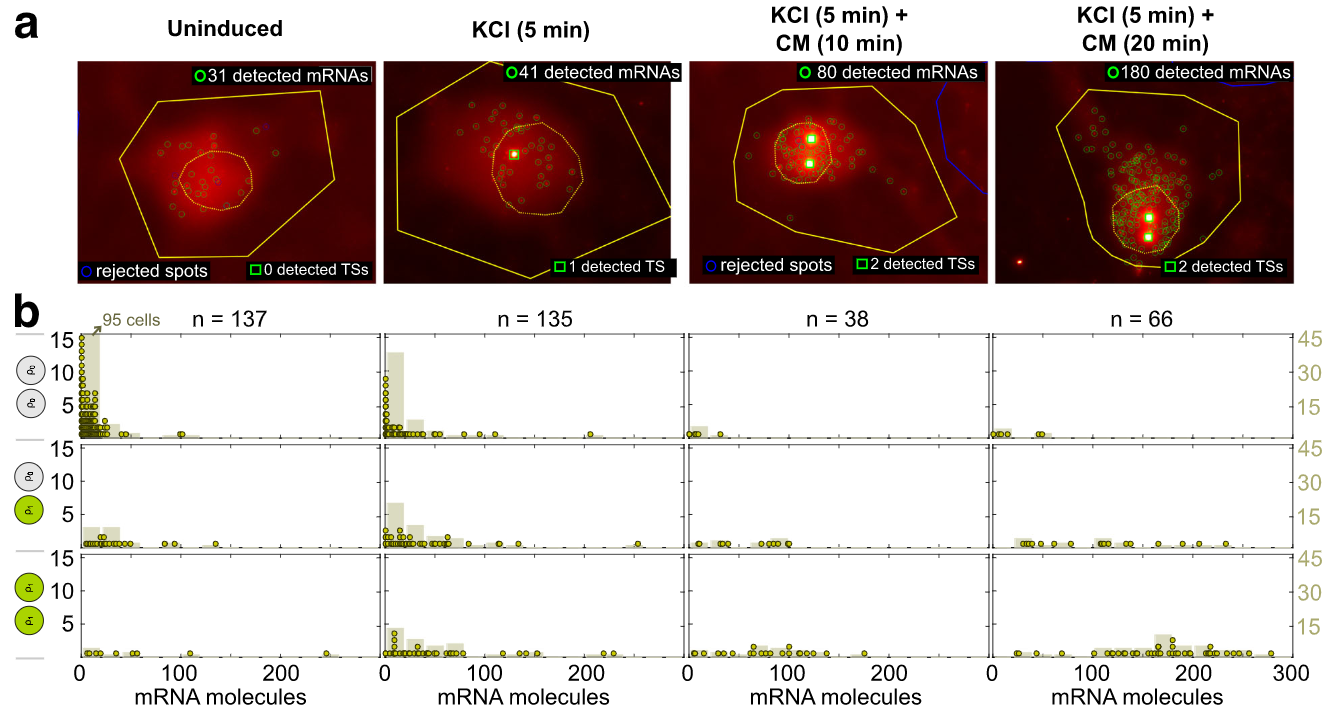
\includegraphics[width=14cm]{figure-1.png}
\end{figure}

\end{frame}

\begin{frame}{Two-state model of gene expression}

\begin{figure}
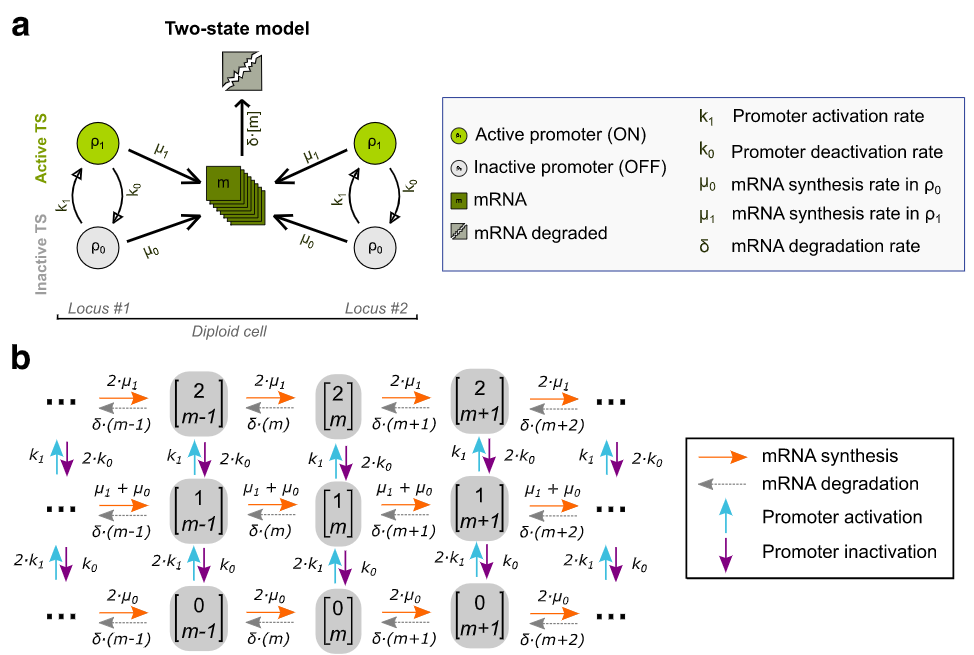
\includegraphics[width=12cm]{figure-2.png}
\end{figure}

\end{frame}

\begin{frame}{Validating BayFish on synthetic smFISH data}

\begin{figure}
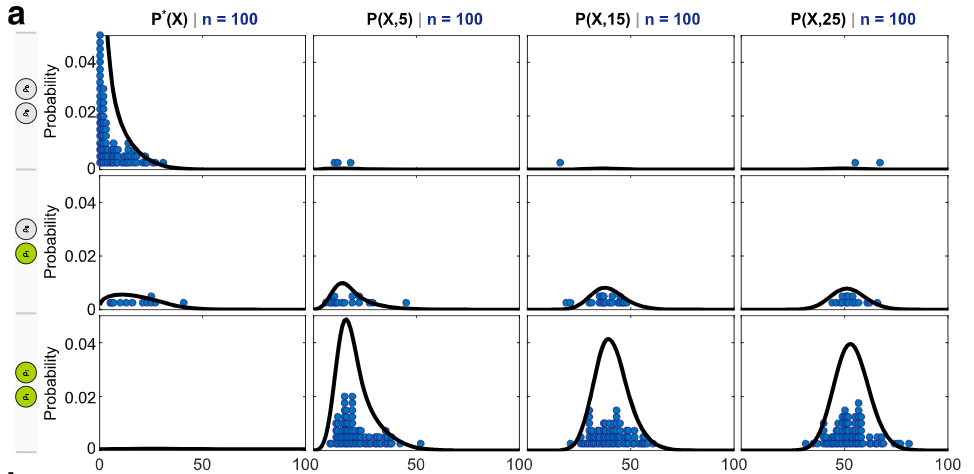
\includegraphics[width=14cm]{figure-3a.png}
\end{figure}

\end{frame}

\begin{frame}{Validating BayFish on synthetic smFISH data}

\begin{figure}
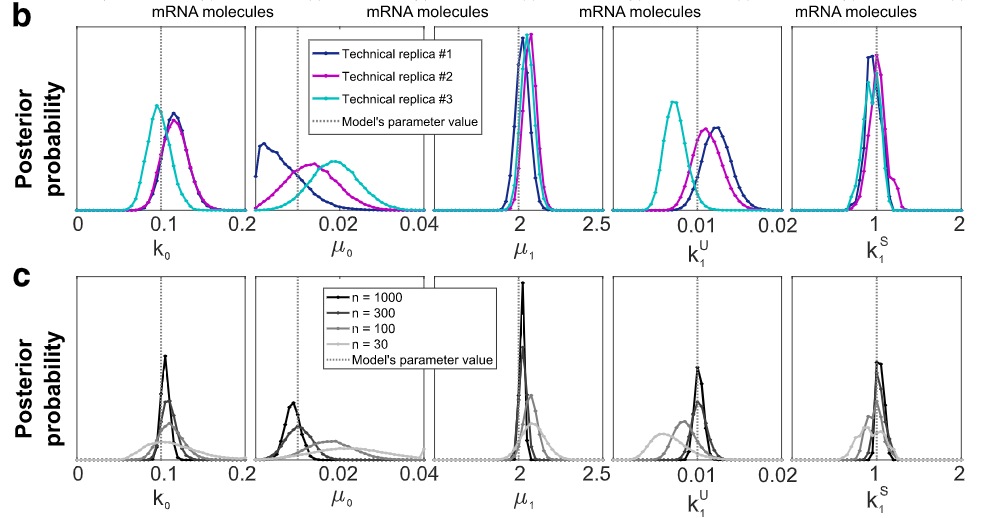
\includegraphics[width=14cm]{figure-3b.png}
\end{figure}

\end{frame}

\begin{frame}{Model selection using BayFish and information criteria}

\begin{figure}
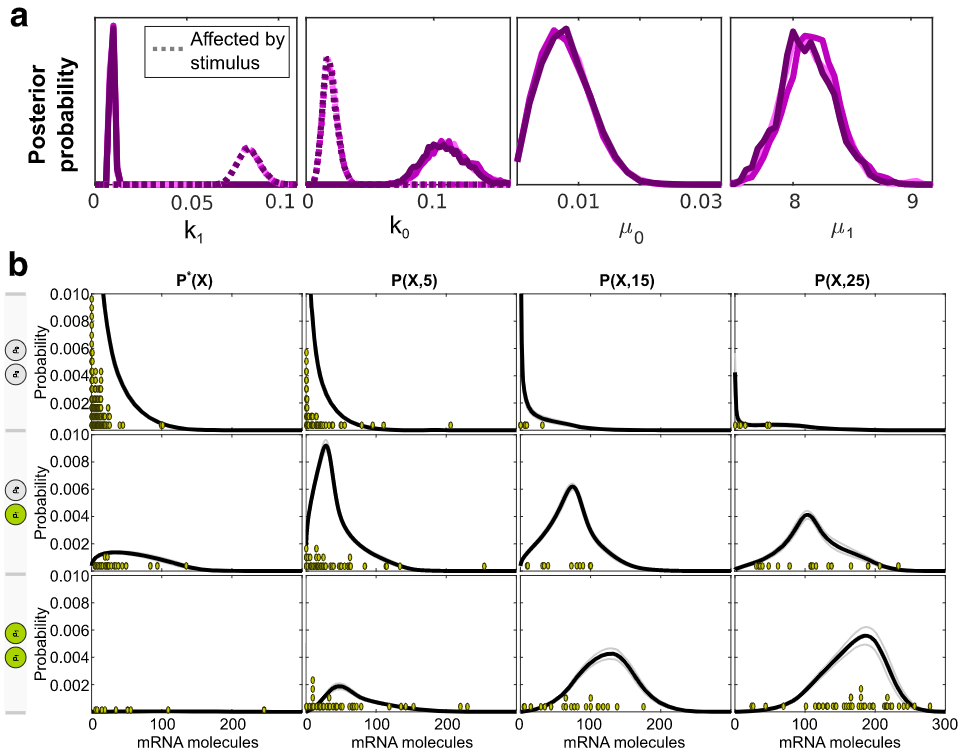
\includegraphics[width=10cm]{figure-4.png}
\end{figure}

\end{frame}

\begin{frame}{Bayesian posterior distribution for (k1,k0)-stimulus model run on Npas4 data}

\begin{figure}
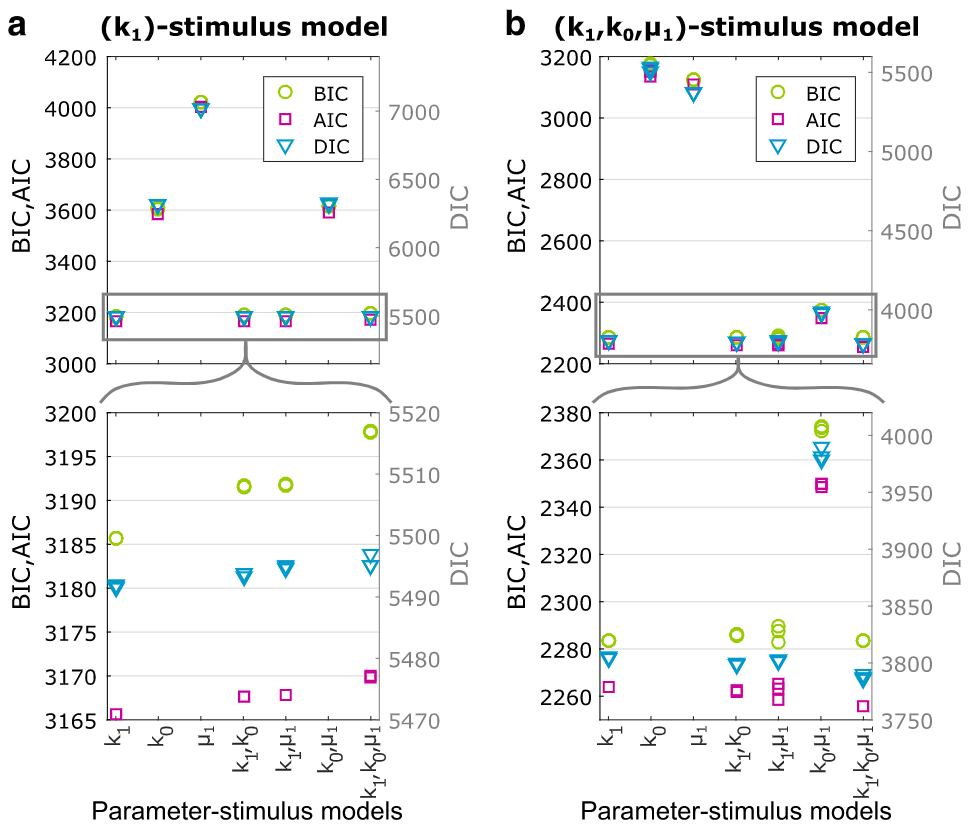
\includegraphics[width=9cm]{figure-5.png}
\end{figure}

\end{frame}


\end{document}